\scanpage{187}
des $G_{\mathbf R}$-modules de dim finie sur $\mathbf R$. Le cône qui exprime cette effectivité est \uline{engendré} par les \deleted{$u(s')$} rayons définis par les $v(s')$. C'est un fait qui exprime \inserted{\figure{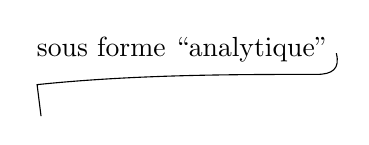
\begin{tikzpicture}[x=1cm,y=1cm]\node at (0,.35) {sous forme ``analytique''};\draw (-1.8,-.5)--(-1.85,-.1) .. controls (-.6,.03) and (.7,.03) .. (1.7,.03) .. controls (1.9,.03) and (2,.1) .. (1.95,.3);\end{tikzpicture}}} le fait que les frobénius $f(s')\in G_{\mathbf R}^{\zeta(s')}(\mathbf R)$ ont la vertu que leurs valeurs propres, dans tte représentation de $G_{\mathbf R}^{\zeta(s')}\deleted{(\mathbf R)}$ -- et en fait $=$ de $G_{\deleted{\mathbf R}\mathbf C}^{\zeta(s')}$ -- sont des \uline{entiers} algébriques, ce qui est une condition arithmétique assez draconienne !
\margin{186}
